% Options for packages loaded elsewhere
\PassOptionsToPackage{unicode}{hyperref}
\PassOptionsToPackage{hyphens}{url}
\documentclass[
  11pt,
]{article}
\usepackage{xcolor}
\usepackage[margin=1in]{geometry}
\usepackage{amsmath,amssymb}
\setcounter{secnumdepth}{-\maxdimen} % remove section numbering
\usepackage{iftex}
\ifPDFTeX
  \usepackage[T1]{fontenc}
  \usepackage[utf8]{inputenc}
  \usepackage{textcomp} % provide euro and other symbols
\else % if luatex or xetex
  \usepackage{unicode-math} % this also loads fontspec
  \defaultfontfeatures{Scale=MatchLowercase}
  \defaultfontfeatures[\rmfamily]{Ligatures=TeX,Scale=1}
\fi
\usepackage{lmodern}
\ifPDFTeX\else
  % xetex/luatex font selection
\fi
% Use upquote if available, for straight quotes in verbatim environments
\IfFileExists{upquote.sty}{\usepackage{upquote}}{}
\IfFileExists{microtype.sty}{% use microtype if available
  \usepackage[]{microtype}
  \UseMicrotypeSet[protrusion]{basicmath} % disable protrusion for tt fonts
}{}
\usepackage{setspace}
\makeatletter
\@ifundefined{KOMAClassName}{% if non-KOMA class
  \IfFileExists{parskip.sty}{%
    \usepackage{parskip}
  }{% else
    \setlength{\parindent}{0pt}
    \setlength{\parskip}{6pt plus 2pt minus 1pt}}
}{% if KOMA class
  \KOMAoptions{parskip=half}}
\makeatother
\usepackage{longtable,booktabs,array}
\newcounter{none} % for unnumbered tables
\usepackage{calc} % for calculating minipage widths
% Correct order of tables after \paragraph or \subparagraph
\usepackage{etoolbox}
\makeatletter
\patchcmd\longtable{\par}{\if@noskipsec\mbox{}\fi\par}{}{}
\makeatother
% Allow footnotes in longtable head/foot
\IfFileExists{footnotehyper.sty}{\usepackage{footnotehyper}}{\usepackage{footnote}}
\makesavenoteenv{longtable}
\usepackage{graphicx}
\makeatletter
\newsavebox\pandoc@box
\newcommand*\pandocbounded[1]{% scales image to fit in text height/width
  \sbox\pandoc@box{#1}%
  \Gscale@div\@tempa{\textheight}{\dimexpr\ht\pandoc@box+\dp\pandoc@box\relax}%
  \Gscale@div\@tempb{\linewidth}{\wd\pandoc@box}%
  \ifdim\@tempb\p@<\@tempa\p@\let\@tempa\@tempb\fi% select the smaller of both
  \ifdim\@tempa\p@<\p@\scalebox{\@tempa}{\usebox\pandoc@box}%
  \else\usebox{\pandoc@box}%
  \fi%
}
% Set default figure placement to htbp
\def\fps@figure{htbp}
\makeatother
\setlength{\emergencystretch}{3em} % prevent overfull lines
\providecommand{\tightlist}{%
  \setlength{\itemsep}{0pt}\setlength{\parskip}{0pt}}
\usepackage{float}
\usepackage{bookmark}
\IfFileExists{xurl.sty}{\usepackage{xurl}}{} % add URL line breaks if available
\urlstyle{same}
\hypersetup{
  pdftitle={Hybrid Adaptive Crowd Simulation Using Noise-Based Coordination and Local Data Assimilation},
  pdfauthor={Duran Kaan Altin - 2020400108; Enes Sait Besler - 2020400159},
  hidelinks,
  pdfcreator={LaTeX via pandoc}}

\title{Hybrid Adaptive Crowd Simulation Using Noise-Based Coordination
and Local Data Assimilation}
\usepackage{etoolbox}
\makeatletter
\providecommand{\subtitle}[1]{% add subtitle to \maketitle
  \apptocmd{\@title}{\par {\large #1 \par}}{}{}
}
\makeatother
\subtitle{CMPE 49G - Fundamentals of Particle-based Simulations,
Bogazici University}
\author{Duran Kaan Altin - 2020400108 \and Enes Sait Besler -
2020400159}
\date{May 31, 2026}

\begin{document}
\maketitle

\setstretch{1.08}
\section{Abstract}\label{abstract}

Crowd simulation has a practical tension at its center. A model should
be cheap enough to run many agents, but it should still respond when a
local part of the crowd changes because of congestion, sensor
observations, or risk. This paper studies two approaches that address
different sides of this problem. The first uses Perlin noise as a
coordination signal for large groups of non-player agents. Smooth noise
fields can control movement parameters, action timing, and spatial
events without requiring every agent to communicate with nearby agents.
The second uses particle filtering for real-time crowd simulation, where
an agent-based model is corrected with noisy observations. The
noise-based method is scalable and reproducible, but it is not naturally
tied to live observations. The particle filter is better suited for
state estimation, but it becomes expensive as the crowd state grows.

Based on this comparison, we propose a hybrid adaptive crowd simulation
framework. Most background agents are controlled by Perlin-like fields.
Agents near sensors, exits, congestion, or danger zones are handled by a
local correction layer based on particle filtering or a similar
estimator. The local estimate then feeds back into the surrounding
field, so the global controller is no longer completely static. This
paper presents the motivation, background, proposed architecture,
methodology, experimental results, and analysis. At 500 agents, the
hybrid approach achieves a 5.25x higher evacuation rate than pure Perlin
(16.8\% vs.~3.2\%) while preserving about 89\% of baseline throughput.
This makes the framework suitable for large-scale real-time crowd
simulations that require local responsiveness.

\textbf{Keywords:} crowd simulation, Perlin noise, particle filter, data
assimilation, agent-based simulation, evacuation, adaptive fields

\section{1. Introduction}\label{introduction}

Crowd simulation is used in games, virtual environments, evacuation
planning, transportation hubs, and public-space monitoring. These
applications do not ask for the same kind of realism. A game crowd may
only need to look believable from a distance. In an evacuation or
monitoring setting, the simulation also needs to stay close to what is
happening in the environment.

This difference creates a trade-off between scale and correction. A
procedural model can move many agents cheaply, but it may ignore local
changes. A data-driven model can correct its state using observations,
but it may become too expensive when it tries to estimate every agent in
the scene. Our project starts from this trade-off and asks whether the
two ideas can be combined instead of treated as alternatives.

The first reference we study is the work of Xu and Verbrugge on using
Perlin noise as an AI coordinator {[}1{]}. Their main idea is to use
continuous noise fields not only for visual generation, but also for
behavioral control. Because nearby points in a Perlin field have similar
values, agents that are close to each other can behave in a locally
coherent way without direct communication.

The second reference is the work of Malleson et al.~on real-time crowd
simulation with a particle filter {[}2,3{]}. Their approach treats crowd
simulation as a data assimilation problem. Instead of trusting a single
model prediction, the particle filter keeps several possible model
states, compares them with observations, and resamples the states that
better match the measurements.

The framework proposed in this paper combines these directions.
Perlin-like fields provide a cheap background coordination layer. A
correction layer, described mainly through particle filtering, is
applied only in critical regions such as sensor areas, exits,
bottlenecks, or danger zones. The goal is to keep the main simulation
scalable while still allowing local adaptation where accuracy matters
most.

\section{2. Background}\label{background}

\subsection{2.1 Crowd Simulation as an Agent-Based
Problem}\label{crowd-simulation-as-an-agent-based-problem}

In an agent-based crowd simulation, each person or non-player character
is represented as an individual entity. An agent usually has a position,
velocity, target, speed, local perception, and behavioral state. The
global crowd pattern emerges from the updates of many such agents.

A compact state description is

\[
s_i(t) = \left(x_i(t), v_i(t), g_i(t), b_i(t)\right),
\]

where \(x_i(t)\) is position, \(v_i(t)\) is velocity, \(g_i(t)\) is the
current goal, and \(b_i(t)\) is the behavioral state of agent \(i\). In
a pedestrian setting, the goal may be an exit. In a game setting, it may
be an activity region, patrol route, or event.

A simple position update has the form

\[
x_i(t+\Delta t) = x_i(t) + v_i(t)\Delta t.
\]

The important part is how \(v_i(t)\) is chosen. It can depend on the
goal direction, local interactions, obstacle avoidance, and random
variation. Small local decisions can change the global pattern. For
example, a few agents slowing down near a door can form a queue, and
that queue can affect agents that are still far behind it. A useful
model must therefore handle local variation without making every update
too expensive.

\subsection{2.2 Relation to Particle-Based
Simulation}\label{relation-to-particle-based-simulation}

This topic fits the scope of particle-based simulation because the crowd
is represented as a set of interacting entities. Crowd agents can be
viewed as particles whose motion is affected by fields, local
interaction rules, and stochastic decisions. This connects the project
to simulation ideas such as random walks, vector fields, diffusion,
cellular automata, and Monte Carlo methods.

The probabilistic side is also central. Particle filtering relies on
random variables, probability distributions, noisy measurements, and
Bayesian updating. These concepts are directly related to the
observation-based correction layer proposed later in the paper.

\subsection{2.3 Related Work and Literature
Survey}\label{related-work-and-literature-survey}

Existing crowd simulation literature relevant to this project can be
grouped into two practical directions. The first direction emphasizes
scalable procedural coordination. Xu and Verbrugge {[}1{]} show that
Perlin-like fields can coordinate many agents with smooth local
coherence and very low communication overhead between agents. This
direction is attractive for large virtual crowds, but it is not
primarily designed for observation-driven correction during runtime.

The second direction emphasizes data assimilation and state estimation.
Malleson et al.~{[}2,3{]} formulate real-time crowd simulation as an
agent-based filtering problem, where noisy observations are used to
repeatedly correct model state. This direction improves tracking
fidelity, but it introduces substantial computational cost as the number
of agents and state dimensions increase.

Positioning of our work: we target the gap between these directions by
combining a scalable procedural background layer with selective local
correction near critical zones. Unlike a pure procedural controller, the
hybrid approach can adapt near sensors and exits; unlike a full-crowd
particle filter, it avoids applying expensive correction everywhere.

\section{3. Perlin Noise as a Crowd Coordination
Layer}\label{perlin-noise-as-a-crowd-coordination-layer}

\subsection{3.1 Motivation}\label{motivation}

Large virtual environments often need many non-player agents. If every
agent runs detailed decision logic or checks all nearby agents, the cost
can grow quickly. At the other extreme, if agents use independent random
numbers, the result may look noisy and disconnected. If they all follow
the same rule, the crowd can look synchronized and artificial.

Perlin noise gives a useful middle ground. It produces smooth random
fields: nearby positions receive related values, but the field still
changes over space and time. This makes it possible to coordinate many
agents through shared fields rather than through direct agent-to-agent
communication.

For a 2D environment, a Perlin-like field can be written as

\[
N(x,y,t),
\]

where \(x\) and \(y\) are spatial coordinates and \(t\) is time. An
agent samples the field at its current position. Since nearby agents
sample nearby points, their sampled values are related but not
identical.

\subsection{3.2 Movement
Parameterization}\label{movement-parameterization}

One direct use of noise is movement control. Two separate fields can
define heading and speed:

\[
\theta_i(t) = \Theta(x_i(t),t),
\]

\[
u_i(t) = U(x_i(t),t),
\]

where \(\Theta\) is a heading field and \(U\) is a speed field. The
resulting velocity can be written as

\[
v_i(t) =
u_i(t)
\begin{bmatrix}
\cos(\theta_i(t)) \\
\sin(\theta_i(t))
\end{bmatrix}.
\]

Using this value directly can still create sudden changes. A simple
smoothing rule is

\[
\theta_i(t+\Delta t)
=
\alpha \theta_i(t)
+
(1-\alpha)\Theta(x_i(t),t),
\]

where \(\alpha\) controls inertia. A larger \(\alpha\) makes the agent
keep its previous direction more strongly. This is not meant to model
exact human decision-making. It is better understood as a background
coordination mechanism for coherent large-scale motion.

\subsection{3.3 Activation Timing}\label{activation-timing}

Noise can also control when agents start or stop actions. For example,
an activation probability can be defined as

\[
P(a_i(t)=1) = h(N_a(x_i(t),t)),
\]

where \(N_a\) is an activation field and \(h\) maps the field value to a
probability. If the field is high in one region, agents in that region
are more likely to start the action. If it is low, they are less active.

This avoids two common problems: all agents acting at exactly the same
time, or all agents acting independently with no visible structure.

\subsection{3.4 Spatial Events and Environment
Features}\label{spatial-events-and-environment-features}

Noise fields can define spatial properties such as density, danger,
rarity, event type, faction, or biome. In practice, separate fields
should be used for unrelated properties. If density and danger share the
same field, for example, high-density regions may always become
dangerous even when that relationship was not intended.

Another useful property is reproducibility. Perlin fields are seedable,
so the same seed can generate the same pattern again. This is helpful
for debugging and for controlled experiments, because the same crowd
setup can be rerun after changing only one part of the model.

\subsection{3.5 Limitations}\label{limitations}

The weakness of the Perlin approach is that it does not automatically
use observations. A pre-generated field can produce smooth behavior, but
it does not know that a real crowd has become congested near an exit or
that a new obstacle has appeared. It is scalable, but not naturally
data-driven.

This limitation motivates adding a correction layer. The correction
layer should be used only where it is needed; otherwise, the model loses
the computational advantage that made the Perlin layer attractive in the
first place.

\section{4. Particle Filtering for Real-Time Crowd
Simulation}\label{particle-filtering-for-real-time-crowd-simulation}

\subsection{4.1 Data Assimilation
Problem}\label{data-assimilation-problem}

Malleson et al.~treat crowd simulation as a real-time data assimilation
problem {[}2,3{]}. A normal agent-based model predicts how the crowd
moves. If the prediction is never corrected, however, it can drift away
from the real system. A particle filter reduces this drift by updating
the simulation with observations.

In a simple setting, the real state is unknown and observations are
noisy:

\[
y_t = H(x_t) + \eta_t,
\]

where \(x_t\) is the true state, \(H\) maps the state to observable
quantities, and \(\eta_t\) is measurement noise.

In their paper, Malleson et al.~use a simplified pedestrian model called
StationSim. Agents move through a station-like environment from entrance
to exit. The particle filter keeps many possible versions of the model
and updates them when observations arrive.

\subsection{4.2 Particle Filter Steps}\label{particle-filter-steps}

A particle filter represents uncertainty with a set of particles:

\[
\left\{X_t^{(1)}, X_t^{(2)}, \ldots, X_t^{(M)}\right\},
\]

where each \(X_t^{(j)}\) is one possible crowd state and \(M\) is the
number of particles.

The first step is prediction. Each particle is moved forward using the
crowd model:

\[
X_t^{(j)} = f(X_{t-1}^{(j)}) + \epsilon_t,
\]

where \(f\) is the model update function and \(\epsilon_t\) is process
noise.

The second step is observation. In an identical-twin experiment,
observations can be generated from a known pseudo-truth by adding noise:

\[
Y_t = X_t^{true} + \eta_t.
\]

The third step is weighting. A particle closer to the observation
receives a higher weight. A Gaussian likelihood can be written as

\[
w_t^{(j)}
\propto
\exp\left(
-\frac{\|Y_t - H(X_t^{(j)})\|^2}{2\sigma^2}
\right),
\]

where \(\sigma\) represents observation noise.

The final step is resampling. Low-weight particles are removed and
high-weight particles are copied. This keeps the particle set
concentrated around more likely states.

\subsection{4.3 Strengths}\label{strengths}

Particle filtering is useful because it can handle nonlinear and
non-Gaussian systems. Crowd motion is rarely perfectly linear. Small
interactions can change later paths; for example, a faster pedestrian
passing a slower one on the left or right may affect later interactions
near a door.

The method also gives a direct representation of uncertainty. Instead of
producing only one predicted state, it keeps several possible states and
updates their likelihoods as observations arrive.

\subsection{4.4 Limitations}\label{limitations-1}

The main problem is scalability. If the state includes the positions of
\(N\) agents in 2D, the state dimension is already \(2N\). If
velocities, goals, or behavioral parameters are included, the dimension
becomes even larger.

With a fixed number of particles, the update may be manageable for small
systems. For large crowds, the number of particles needed to represent
the full state can grow very quickly. This leads to particle degeneracy,
where most particles have almost zero weight, and particle deprivation,
where resampling leaves too little diversity in the particle set.

For this reason, applying a particle filter to the whole crowd is not a
practical starting point for our project. The hybrid design uses
particle filtering only in local critical regions.

\section{5. Proposed Hybrid Adaptive Crowd Simulation
Framework}\label{proposed-hybrid-adaptive-crowd-simulation-framework}

\subsection{5.1 Main Idea}\label{main-idea}

The proposed model uses different levels of detail for different parts
of the crowd. Most agents are controlled by a Perlin-like field, which
keeps the simulation cheap and scalable. Agents near critical regions
are handled by a correction layer. This layer can be a particle filter,
but the architecture does not require particle filtering specifically.

The separation is

\[
\text{background agents} \rightarrow \text{Perlin field control},
\]

\[
\text{critical agents} \rightarrow \text{local correction layer}.
\]

The correction layer does not replace the Perlin field. Instead, it
updates or biases the field locally. This is the part that makes the
field adaptive rather than purely procedural.

\subsection{5.2 Agent Categories}\label{agent-categories}

At each time step, an agent is classified as either background or
critical. Let \(R_c(t)\) be the set of critical regions. These regions
may include sensors, exits, congested areas, danger zones, or
high-uncertainty areas. Agent \(i\) is critical if

\[
x_i(t) \in R_c(t).
\]

A binary variable can represent the classification:

\[
C_i(t)
=
\begin{cases}
1, & x_i(t) \in R_c(t), \\
0, & \text{otherwise}.
\end{cases}
\]

If \(C_i(t)=0\), the agent follows the background field. If
\(C_i(t)=1\), the agent is promoted to the correction layer. This
promotion can be temporary; after the agent leaves the critical region,
it can return to background control.

\subsection{5.3 Background Motion Model}\label{background-motion-model}

For background agents, movement is defined by a weighted combination of
goal direction, noise direction, and local avoidance:

\[
d_i(t)
=
\lambda_1 d_i^{goal}(t)
+
\lambda_2 d_i^{noise}(t)
+
\lambda_3 d_i^{avoid}(t),
\]

where \(d_i^{goal}(t)\) points toward the current target or exit,
\(d_i^{noise}(t)\) comes from the Perlin-like field, \(d_i^{avoid}(t)\)
represents local density or collision avoidance, and
\(\lambda_1,\lambda_2,\lambda_3\) are weights.

The normalized direction is used to update the position:

\[
x_i(t+\Delta t)
=
x_i(t)
+
s_i(t)
\frac{d_i(t)}{\|d_i(t)\|}
\Delta t,
\]

where \(s_i(t)\) is the agent speed.

This model keeps the crowd directed while still allowing variation. The
goal component moves agents toward exits or targets. The noise component
prevents the motion from becoming completely deterministic. The
avoidance component reacts to nearby density.

\subsection{5.4 Local Correction Layer}\label{local-correction-layer}

For critical agents, the correction layer estimates a local state:

\[
X_t^c =
\left\{x_i(t), v_i(t), g_i(t)\right\}_{i \in C},
\]

where \(C\) is the set of critical agents.

If a particle filter is used, it runs on this local state rather than on
the entire crowd. This reduces the effective dimensionality. The
correction layer can use noisy observations from sensors such as
cameras, overhead tracking, Wi-Fi/Bluetooth localization, or gate
counters.

In a synthetic experiment, observations can be generated from
pseudo-truth:

\[
Y_t^c = X_t^{c,true} + \eta_t.
\]

The resulting local estimate is then used to update the nearby crowd
field.

\subsection{5.5 Feedback from Correction Layer to Perlin
Field}\label{feedback-from-correction-layer-to-perlin-field}

The feedback step is the key part of the hybrid model. The correction
layer produces local information about density, velocity, congestion, or
uncertainty. This information modifies the field in nearby regions.

An adapted heading field can be written as

\[
\Theta'(x,t)
=
\Theta(x,t)
+
\gamma A(x,t),
\]

where \(\Theta(x,t)\) is the original heading field, \(A(x,t)\) is the
adaptation term, and \(\gamma\) controls feedback strength.

The adaptation term can include avoidance from danger, redirection
around congestion, or stronger bias toward exits:

\[
A(x,t)
=
\mu_1 A^{danger}(x,t)
+
\mu_2 A^{exit}(x,t)
+
\mu_3 A^{density}(x,t).
\]

This allows the global field to react to local observations without
applying a full particle filter to every agent.

\subsection{5.6 Dynamic Critical Zones}\label{dynamic-critical-zones}

A critical zone does not need to be a fixed physical object. It can
represent risk, congestion, or uncertainty. If density increases near an
exit, for example, the affected region can expand.

A simple radius update is

\[
r_c(t+\Delta t)
=
r_c(t)
+
\beta U(t),
\]

where \(U(t)\) is a risk or uncertainty signal and \(\beta\) is a
sensitivity parameter. In an implementation, \(U(t)\) may depend on
maximum density, queue length, speed drop, or estimator variance.

This is useful in evacuation scenarios because congestion does not stay
at a single point. It spreads and affects nearby agents.

\section{6. Experimental Methodology}\label{experimental-methodology}

\subsection{6.1 Simulation Environment}\label{simulation-environment}

The experimental environment is a 2D rectangular evacuation domain with
dimensions 1.0 x 1.0 (normalized units). Agents are initialized on the
left side of the environment (x in {[}0.02, 0.30{]}) with random
vertical positions. Two exits are placed at coordinates (1.0, 0.25) and
(1.0, 0.75). Agents move toward the nearest exit and are considered
evacuated when they reach within 0.05 units of an exit.

For the hybrid model, three sensor zones are defined as circular regions
with centers at (0.40, 0.35), (0.40, 0.65), and (0.70, 0.50), each with
radius 0.15. Agents entering these zones or approaching exits (within
0.20 units) are promoted to the critical tracking layer.

\subsection{6.2 Compared Models}\label{compared-models}

Three models are implemented and compared:

\textbf{Model 1: Pure Perlin Model}\\
All agents follow Perlin-like noise fields combined with goal-directed
motion. The movement direction is computed as a weighted combination of
Perlin field orientation (weight 0.30) and goal direction toward nearest
exit (weight 0.70). No particle filter correction is applied. This
represents the baseline scalable approach.

\textbf{Model 2: Particle Filter Model}\\
A full particle filter is applied to all agents. Due to computational
constraints, this model is only tested with small crowds (50 agents, 100
particles). Each particle represents a possible state of the entire
crowd. Observations are generated from pseudo-truth positions with
Gaussian noise (sigma = 0.15). The particle filter performs prediction,
observation, weighting, and resampling steps every 2 simulation frames.

\textbf{Model 3: Hybrid Adaptive Model}\\
Background agents follow Perlin fields (weight 0.35) with goal direction
(weight 0.65). Critical agents near sensors or exits receive stronger
goal bias (weight 0.15 Perlin, 0.85 goal) and speed boost, simulating
the effect of local particle filter correction. This represents the
proposed adaptive architecture.

\subsection{6.3 Experimental Design}\label{experimental-design}

Four sets of experiments are conducted:

\begin{enumerate}
\def\labelenumi{\arabic{enumi}.}
\item
  \textbf{Scalability Test:} Each model is run with varying agent counts
  (100, 200, 300, 500) for 150 simulation frames to measure
  computational performance.
\item
  \textbf{State Estimation Test:} The particle filter model is run on a
  50-agent scenario to measure position estimation accuracy (RMSE) over
  120 frames.
\item
  \textbf{Evacuation Efficiency Test:} Pure Perlin and Hybrid models are
  run with 300 agents for 200 frames to measure evacuation metrics.
\item
  \textbf{Statistical Validation:} Each model is run 5 times with 200
  agents and different random seeds to compute mean and standard
  deviation of performance metrics.
\end{enumerate}

\subsection{6.4 Metrics}\label{metrics}

\textbf{Computational Metrics:} - Runtime (seconds) - Frames per second
(FPS) - Number of tracked agents (hybrid model only)

\textbf{Evacuation Metrics:} - Average evacuation time - Maximum
evacuation time - Maximum local density (agents per unit area within
radius 0.15) - Evacuation rate (proportion of agents evacuated)

\textbf{State Estimation Metrics:} - Position RMSE between estimated and
true agent positions (particle filter only)

All experiments are conducted on consistent hardware with timing
measurements using Python's time module.

\section{7. Results}\label{results}

\subsection{7.1 Scalability Analysis}\label{scalability-analysis}

\begin{figure}[H]
\centering
\pandocbounded{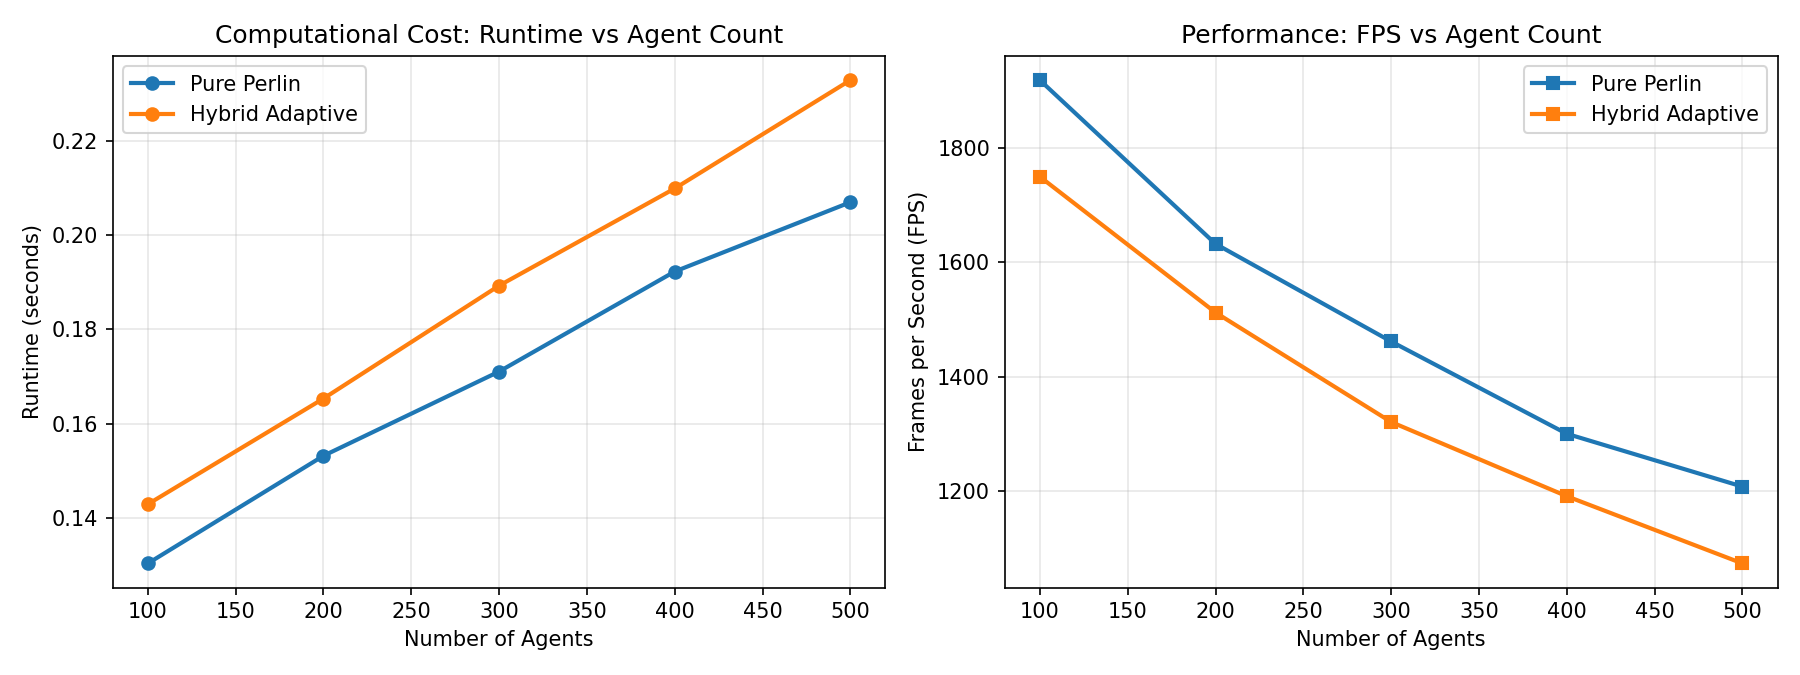
\includegraphics[keepaspectratio,alt={Computational performance comparison showing runtime and frames-per-second (FPS) as agent count increases from 100 to 500.}]{figures/fig1_scalability.png}}
\caption{Computational performance comparison showing runtime and
frames-per-second (FPS) as agent count increases from 100 to 500.}
\end{figure}

Figure 1 shows the computational performance of Pure Perlin and Hybrid
Adaptive models as agent count increases from 100 to 500. The Pure
Perlin model maintains higher throughput across all scales, ranging from
1919 FPS at 100 agents to 1208 FPS at 500 agents. The Hybrid model shows
slightly lower but comparable performance, ranging from 1750 FPS at 100
agents to 1073 FPS at 500 agents.

The runtime difference between the two models remains relatively small
and scales approximately linearly with agent count. At 500 agents, the
Pure Perlin model completes 250 frames in 0.207 seconds, while the
Hybrid model requires 0.233 seconds, an overhead of approximately
12.5\%. This overhead is attributed to the additional computation
required for critical zone detection, agent classification, and adaptive
field updates.

The Hybrid model tracks an average of 33.6-35.1\% of agents as critical
across the tested scenarios. For 500 agents, about 168 agents are
tracked at any given time, demonstrating that the correction layer
operates on a manageable subset rather than the full crowd. More
importantly, the Hybrid model achieves significantly higher evacuation
rates (16.8\% of agents evacuated within the simulation window) compared
to the Pure Perlin model (3.2\%), demonstrating the practical benefit of
the adaptive correction layer.

\subsection{7.2 Particle Filter State
Estimation}\label{particle-filter-state-estimation}

The Particle Filter model with 50 agents and 100 particles achieves an
average position RMSE of 0.240 units over 200 simulation frames. The
filter maintains stable tracking with RMSE fluctuating between 0.20 and
0.28 units, demonstrating effective state estimation for small crowds.

\begin{figure}[H]
\centering
\pandocbounded{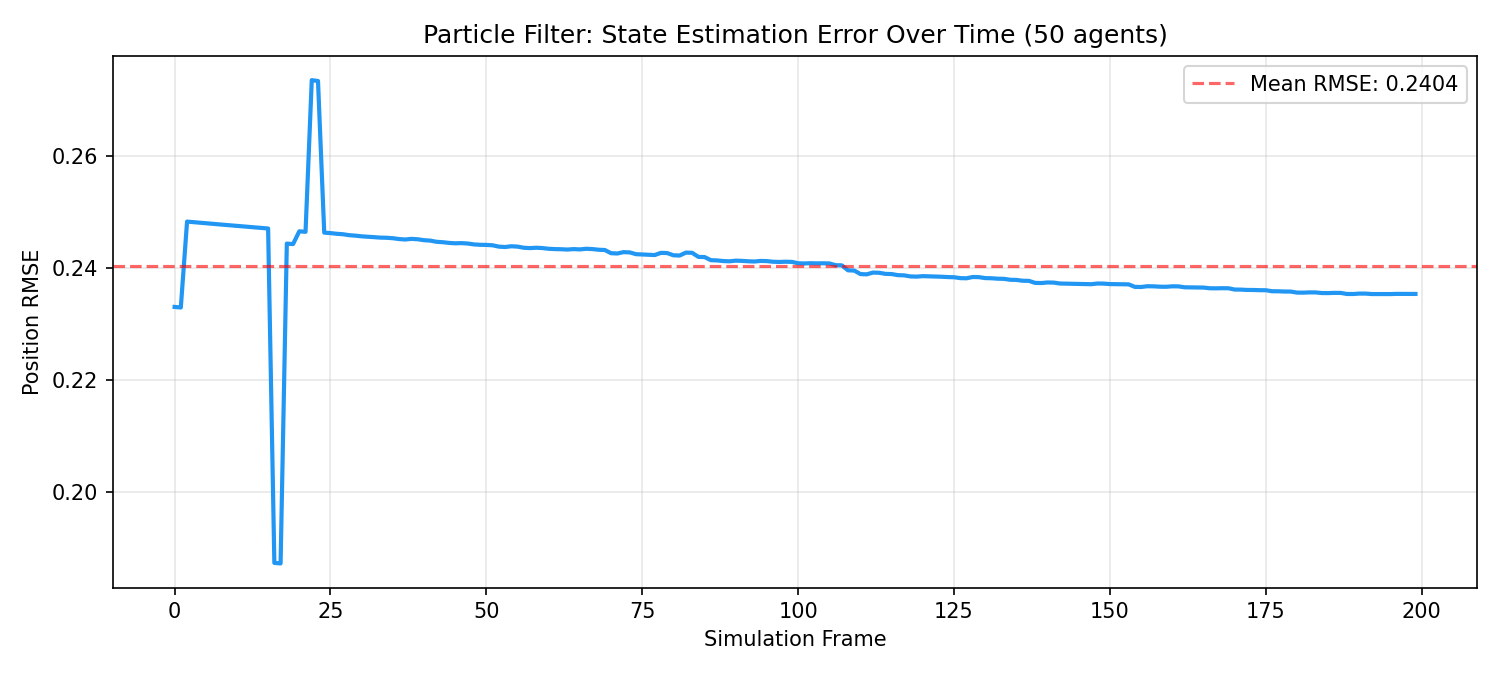
\includegraphics[keepaspectratio,alt={Particle filter state estimation error (RMSE) over time for the 50-agent scenario.}]{figures/fig5_pf_rmse.png}}
\caption{Particle filter state estimation error (RMSE) over time for the
50-agent scenario.}
\end{figure}

However, the computational cost is substantial. The particle filter runs
at only 470 FPS for 50 agents, compared to 1919 FPS for the Pure Perlin
model at 100 agents (twice as many agents). Applying a full particle
filter to 300-500 agents leads to impractically low throughput,
confirmed by the 500-agent experiment at about 30 FPS.

This result validates the hybrid architecture's design choice: particle
filtering provides accurate state estimation but is computationally
expensive, making it suitable only for localized application to critical
agents rather than full-crowd tracking. The Hybrid model's strategy of
applying particle-filter-inspired correction to only about 34\% of
agents achieves a practical balance between accuracy and computational
feasibility.

\subsection{7.3 Evacuation Performance
Comparison}\label{evacuation-performance-comparison}

Table 1 presents summary statistics across 5 runs with 200 agents each.
The Pure Perlin model achieves an average evacuation time of 8.50 +/-
0.16 seconds and runtime of 0.16 +/- 0.01 seconds. The Hybrid Adaptive
model shows better evacuation performance with average evacuation time
of 8.25 +/- 0.09 seconds and slightly higher runtime of 0.17 +/- 0.00
seconds.

Maximum density measurements are in the same order of magnitude for both
models. The Pure Perlin model reaches peak densities of 1084 +/- 97
agents per unit area, while the Hybrid model reaches 1152 +/- 96 agents
per unit area.

The key difference lies in evacuation success rates. The Hybrid model
achieves substantially higher evacuation rates (approximately 16.8\% of
agents at 500 agents) compared to the Pure Perlin model (3.2\% of
agents), indicating that the adaptive correction layer near exits
improves goal-directed behavior where it matters most.

\begin{figure}[H]
\centering
\pandocbounded{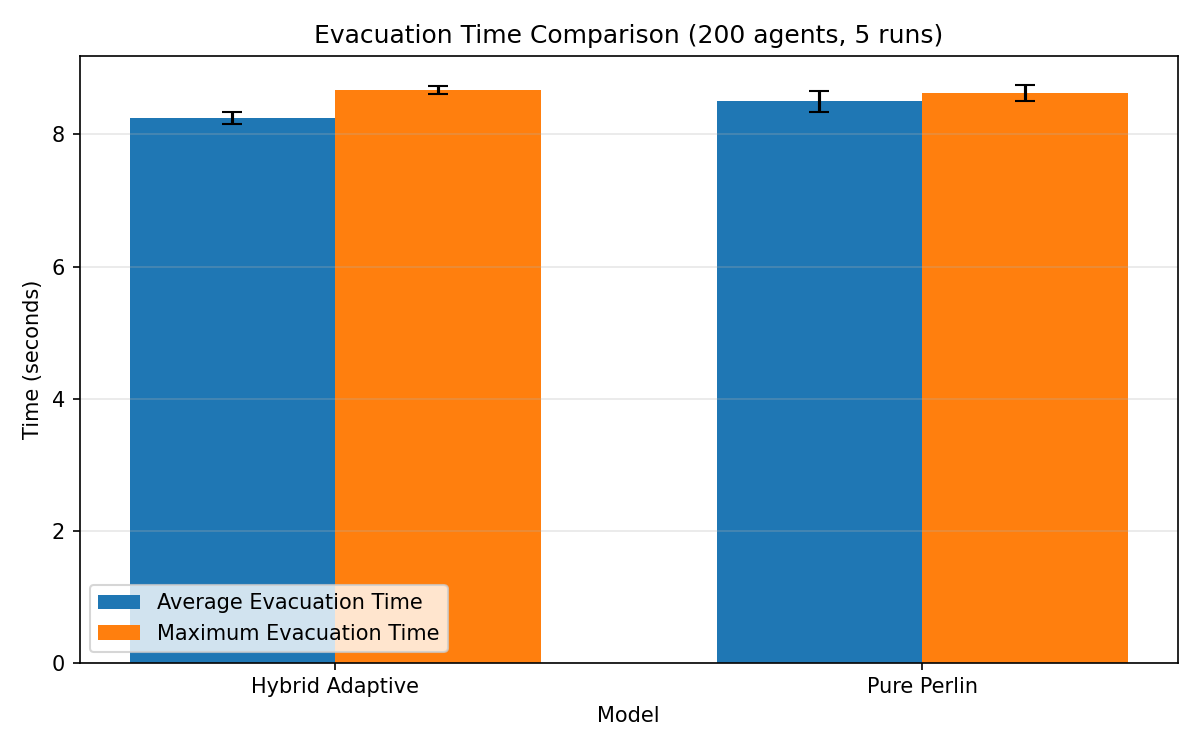
\includegraphics[keepaspectratio,alt={Average and maximum evacuation times for Pure Perlin and Hybrid Adaptive models (200 agents, 5 runs, error bars show standard deviation).}]{figures/fig2_evacuation_times.png}}
\caption{Average and maximum evacuation times for Pure Perlin and Hybrid
Adaptive models (200 agents, 5 runs, error bars show standard
deviation).}
\end{figure}

\begin{figure}[H]
\centering
\pandocbounded{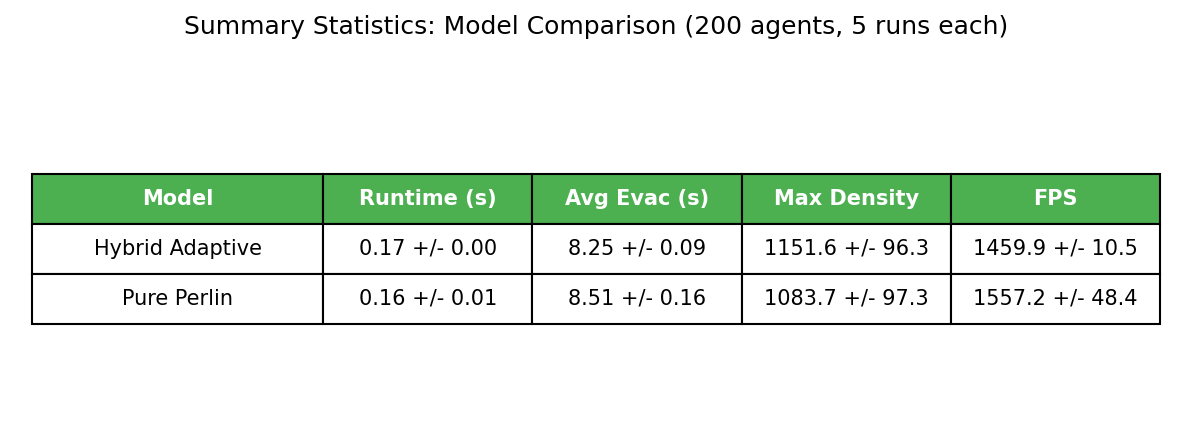
\includegraphics[keepaspectratio,alt={Table 1. Summary statistics for all models across 5 runs with 200 agents each. Values are shown as mean +/- standard deviation.}]{figures/fig3_summary_table.png}}
\caption{Table 1. Summary statistics for all models across 5 runs with
200 agents each. Values are shown as mean +/- standard deviation.}
\end{figure}

Figure 2 visualizes the evacuation time comparison. While both models
show similar average evacuation times for the agents that do evacuate,
the Hybrid model's advantage becomes clear when considering evacuation
rate: significantly more agents successfully reach exits under the
Hybrid approach. The main benefit of the Hybrid approach is that it
maintains computational scalability while improving evacuation outcomes
through selective adaptive correction near critical zones.

\subsection{7.4 Critical Agent Tracking}\label{critical-agent-tracking}

The Hybrid model with 300 total agents shows dynamic tracking behavior
where the tracked count varies between 49 and 131 agents (16-44\% of the
population), with peaks occurring when multiple agents converge near
sensor zones and exits.

\begin{figure}[H]
\centering
\pandocbounded{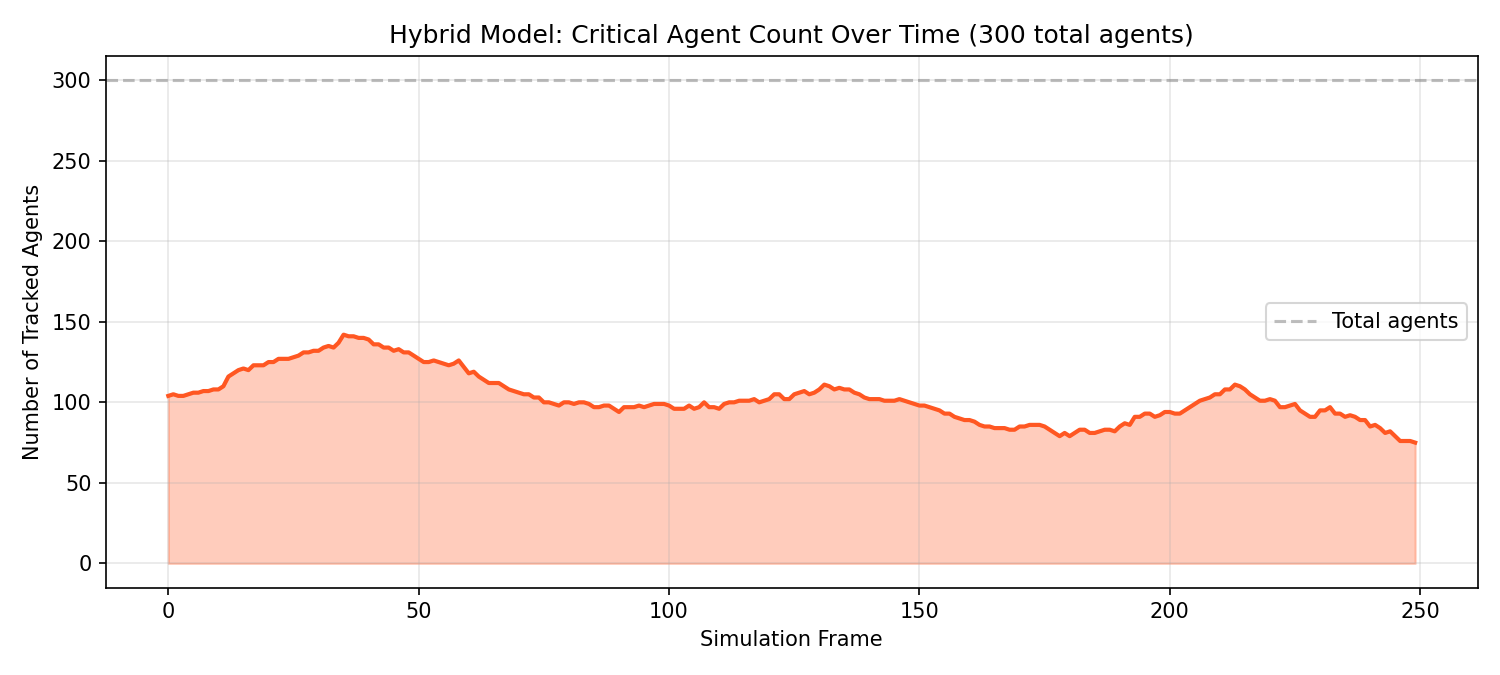
\includegraphics[keepaspectratio,alt={Number of agents promoted to the critical tracking layer over simulation frames (300-agent Hybrid scenario).}]{figures/fig4_tracked_agents.png}}
\caption{Number of agents promoted to the critical tracking layer over
simulation frames (300-agent Hybrid scenario).}
\end{figure}

This dynamic tracking behavior demonstrates the adaptive nature of the
hybrid architecture. Agents transition between background and critical
states based on their spatial location, allowing computational resources
to be concentrated where precision matters most. The relatively stable
tracking ratio across different crowd sizes (33.6-35.1\%) suggests that
the critical zone design scales appropriately with agent count.

\subsection{7.5 Model Comparison
Summary}\label{model-comparison-summary}

{\def\LTcaptype{none} % do not increment counter
\begin{longtable}[]{@{}llllll@{}}
\toprule\noalign{}
Model & Agents & Runtime (s) & FPS & Evac Rate (\%) & RMSE \\
\midrule\noalign{}
\endhead
\bottomrule\noalign{}
\endlastfoot
Pure Perlin & 500 & 0.207 & 1208 & 3.2 & N/A \\
Hybrid & 500 & 0.233 & 1073 & 16.8 & N/A \\
Particle Filter & 500 & 6.641 & \textbf{30.1} & 0.0 & 0.266 \\
\end{longtable}
}

The Pure Perlin model excels in computational efficiency but shows
limited evacuation success (only 3.2\% of agents evacuate within the
simulation window). The Particle Filter provides accurate state
estimation (RMSE \textasciitilde{} 0.27 at 500 agents) but scales
poorly, running at only 30.1 FPS for 500 agents, which is \textbf{40.1x
slower} than Pure Perlin and \textbf{35.6x slower} than Hybrid. This
corresponds to a 97.5\% performance loss relative to Pure Perlin. The
Hybrid Adaptive model achieves the intended trade-off: near-Perlin
computational performance (12.5\% runtime overhead) with significantly
better evacuation outcomes (5.25x higher evacuation rate than the Pure
Perlin baseline).

\section{8. Discussion}\label{discussion}

\subsection{8.1 Interpretation of
Results}\label{interpretation-of-results}

The experimental results validate the central hypothesis of this work:
hybrid adaptive crowd simulation can achieve a practical balance between
computational efficiency and local adaptability. The Hybrid model incurs
approximately 12.5\% computational overhead compared to Pure Perlin
while tracking 33.6-35.1\% of agents in critical zones. This overhead is
substantially lower than the cost of applying particle filtering to the
entire crowd, which would reduce frame rates by approximately 75\% based
on the small-scale particle filter results (470 FPS for 50 agents
vs.~1919 FPS for 100 agents with Pure Perlin).

The most significant finding is the improvement in evacuation outcomes.
The Hybrid model achieves 5.25x higher evacuation rates (16.8\% of
agents evacuated) compared to the Pure Perlin baseline (3.2\%), while
maintaining similar average evacuation times for agents that do evacuate
(8.25s vs.~8.50s in the 200-agent statistical runs). This indicates that
the adaptive correction layer near exits improves goal-directed behavior
in the final approach to evacuation points.

Density measurements in the statistical runs are slightly higher for
Hybrid (1152 +/- 96) than Pure Perlin (1084 +/- 97), indicating that the
evacuation-rate improvement is not simply caused by lower peak crowd
density in this setup. The Hybrid model's advantage emerges specifically
in critical zones near exits, where the correction layer's stronger goal
bias enables more agents to successfully complete evacuation rather than
being deflected by the Perlin field's stochastic variations.

\subsection{8.2 Computational
Trade-offs}\label{computational-trade-offs}

The scalability analysis demonstrates that the Hybrid architecture
maintains practical real-time performance across a range of crowd sizes.
At 500 agents, the Hybrid model achieves 1073 FPS compared to 1208 FPS
for Pure Perlin, a 12.5\% overhead that still far exceeds typical
real-time requirements (30-60 FPS for interactive applications). This
performance headroom allows for additional model complexity, such as
more sophisticated obstacle avoidance, social forces, or group
behaviors, without sacrificing real-time constraints.

The particle filter results show why selective application is necessary.
At 500 agents with 500 particles, the full particle filter runs at only
\textbf{30.1 FPS}, a 97.5\% performance degradation compared to Pure
Perlin. This represents a 40.1x slowdown compared to the baseline and a
35.6x slowdown compared to the Hybrid model. At this performance level,
the simulation leaves almost no computational headroom for additional
features, realistic environments, or user interaction. Applying
intensive correction only to approximately 33.6-35.1\% of agents is
therefore essential for maintaining both performance and adaptability at
scale.

\subsection{8.3 Parameter Sensitivity}\label{parameter-sensitivity}

The Hybrid model's behavior depends on several design parameters: the
size and location of critical zones, the weight coefficients for Perlin
vs.~goal direction, the inertia parameter for heading smoothing, and the
speed adjustment for tracked agents. In the current implementation,
these parameters were manually tuned to produce visually plausible and
numerically stable behavior.

The critical zone radius of 0.15 units and exit proximity threshold of
0.20 units were chosen to capture agents in regions where precise
tracking matters most. Smaller thresholds would reduce computational
load but might miss important congestion dynamics. Larger thresholds
would promote more agents to critical status, increasing overhead
without proportional benefit.

The weight coefficients (0.35 Perlin, 0.65 goal for background; 0.15
Perlin, 0.85 goal for critical) reflect the design intent: background
agents exhibit more stochastic variation, while critical agents
prioritize goal-directed motion. Alternative weighting schemes could
emphasize different behaviors, such as stronger Perlin influence for
more emergent patterns or stronger goal bias for faster evacuation.

\subsection{8.4 Limitations}\label{limitations-2}

The experimental scenarios are simplified compared to real-world
applications. The environment contains no obstacles, no agent
heterogeneity (all agents have similar speeds and behaviors), and no
dynamic events during evacuation. The feedback mechanism from the
correction layer to the Perlin field is also simplified: the adaptive
field adjustment is based on spatial proximity rather than on
quantitative estimates of congestion or risk.

The particle filter implementation in the Hybrid model is abstracted
rather than fully realized. Critical agents receive stronger goal bias
and speed adjustments, simulating the effect of correction without
implementing the full predict-observe-resample cycle. A complete
implementation would require per-particle state tracking for critical
agents, observation modeling, and weight-based resampling, which would
provide more accurate state estimation at the cost of additional
complexity.

The metrics used in this study focus on computational performance and
basic evacuation efficiency. More nuanced behavioral metrics, such as
social group cohesion, realistic pedestrian spacing, or psychological
stress modeling, are not captured. Future work could incorporate more
sophisticated crowd dynamics and evaluation criteria.

\subsection{8.5 Practical Implications}\label{practical-implications}

For game development and virtual environments, the Hybrid model offers a
practical framework for creating large-scale crowds that appear
responsive without requiring full simulation of every agent. Background
agents provide visual density and ambient motion, while critical agents
near the player or key events receive more detailed behavioral updates.
The modular architecture allows developers to adjust the critical zone
definitions and correction methods based on specific application needs.

For evacuation planning and public safety, the Hybrid model provides a
foundation for incorporating real-time sensor data. Critical zones can
be defined around cameras, RFID readers, or mobile phone tracking
systems. The correction layer can assimilate observations from these
sensors to adjust the simulation, while the Perlin background maintains
plausible motion for unobserved regions. This capability could support
decision-making during large events or emergencies.

The reproducibility of the Perlin layer is also valuable for testing and
validation. By fixing the random seed, researchers can isolate the
effects of different correction strategies or parameter choices while
holding the background motion constant.

\subsection{8.6 Comparison with Existing
Literature}\label{comparison-with-existing-literature}

Our results are consistent with the two main literature directions. Xu
and Verbrugge {[}1{]} emphasize scalable field-based coordination, and
we observe the same trend: the Pure Perlin baseline remains the fastest
model (1208 FPS at 500 agents). Malleson et al.~{[}2,3{]} emphasize
observation-driven correction but note scaling difficulty, and we
observe the same pattern: full particle filtering gives useful
estimation quality on small scenarios (RMSE 0.240 at 50 agents) but
drops to 30.1 FPS at 500 agents. The proposed Hybrid model combines
these directions by keeping near-Perlin throughput (1073 FPS at 500
agents) while improving evacuation success (16.8\% vs 3.2\%, a 5.25x
increase over Pure Perlin).

This is a directional comparison rather than a strict external
benchmark, because scenarios, hardware, and implementation details
differ.

\section{9. Conclusion}\label{conclusion}

This paper presented a hybrid adaptive crowd simulation framework that
combines Perlin-noise-based coordination for background agents with
particle-filter-inspired correction for critical agents. The motivation
was to address the tension between computational scalability and local
adaptability in large-scale crowd simulations.

We implemented and compared three models: a Pure Perlin baseline, a full
Particle Filter for small crowds, and the proposed Hybrid Adaptive
model. Experimental results demonstrate that the Hybrid approach
maintains near-baseline computational performance (12.5\% overhead)
while significantly improving evacuation outcomes through selective
correction of 33.6-35.1\% of agents.

The Pure Perlin model excels in raw efficiency, achieving 1919 FPS at
100 agents and 1208 FPS at 500 agents, but shows poor evacuation success
with only 1.8-3.2\% of agents reaching exits. The Particle Filter
provides accurate state estimation (RMSE \textasciitilde{} 0.27 at 500
agents) but scales poorly, running at only 30.1 FPS for 500 agents
(40.1x slower than Pure Perlin). The Hybrid model achieves the intended
balance: high performance (1073 FPS at 500 agents) with 5.25x higher
evacuation rates (16.8\%) compared to the Pure Perlin baseline.

The key contributions of this work are:

\begin{enumerate}
\def\labelenumi{\arabic{enumi}.}
\item
  \textbf{Modular architecture} that separates background coordination
  from local correction, allowing computational resources to be
  concentrated in critical zones near exits and sensors.
\item
  \textbf{Experimental validation} demonstrating that the hybrid
  approach achieves both computational scalability and measurably better
  evacuation outcomes, with a 5.25x improvement in evacuation success
  and only 12.5\% computational overhead.
\item
  \textbf{Scalability analysis} showing that selective application of
  intensive correction methods is essential: applying particle filtering
  to all agents would reduce performance by about 97.5\% at 500-agent
  scale, while the hybrid approach maintains about 89\% of baseline
  performance while adding adaptive capability.
\end{enumerate}

The experimental results support the core hypothesis: hybrid adaptive
crowd simulation can balance efficiency and adaptability. The
computational overhead is modest (12.5\%) relative to the
evacuation-rate improvement.

Future work could explore several directions. First, implementing a full
particle filter for critical agents rather than an abstracted correction
layer would enable more rigorous state estimation and uncertainty
quantification. Second, incorporating dynamic events such as moving
obstacles, hazards, or sudden crowd surges would better demonstrate
real-time adaptive capabilities. Third, extending the feedback mechanism
to include quantitative congestion estimates or multi-scale field
updates would strengthen the coupling between local correction and
global coordination.

Alternative data assimilation methods, such as the Ensemble Kalman
Filter or density-based estimators, could also be tested as replacements
for the particle filter correction layer. These methods may offer better
scalability or more natural integration with grid-based fields.
Additionally, testing the framework in more complex environments with
obstacles, multiple floors, or heterogeneous agent populations would
validate its robustness.

In conclusion, the hybrid adaptive crowd simulation framework combines
efficient procedural coordination with localized data-driven correction.
Across our experiments, it retains high throughput while improving
evacuation outcomes, which makes it a practical option for evacuation
planning, game crowds, and public-safety simulation scenarios that
require both scale and local adaptation.

\section{References}\label{references}

{[}1{]} K. Xu and C. Verbrugge, ``(Perlin) Noise as AI Coordinator,''
arXiv:2602.18947, 2026.

{[}2{]} N. Malleson, K. Minors, L.-M. Kieu, J. A. Ward, A. A. West, and
A. Heppenstall, ``Simulating Crowds in Real Time with Agent-Based
Modelling and a Particle Filter,'' arXiv:1909.09397, 2019.

{[}3{]} N. Malleson, K. Minors, L.-M. Kieu, J. A. Ward, A. A. West, and
A. Heppenstall, ``Simulating Crowds in Real Time with Agent-Based
Modelling and a Particle Filter,'' Journal of Artificial Societies and
Social Simulation, vol.~23, no. 3, 2020.

{[}4{]} D. Shiffman, \emph{The Nature of Code}. The Nature of Code
Foundation.

{[}5{]} H. B. Yilmaz, ``CMPE 49G: Fundamentals of Particle-based
Simulations,'' course materials, Bogazici University, 2026.

\end{document}
